
\section{Introduction}

As outlined in \ref{sec:electricity_price_forecasting} different types of models have been investigated for forecasting spot electricity prices. In this work forecasting models should be used that exhibit the following characteristics: 

\begin{itemize}
	\item computationally lightweight
	\item capable of modeling seasonality
	\item capable of recognizing trends in the dataset
	\item good out-of-sample accuracy based on day ahead and real time electricity prices
	\item capable of being part of an automated model generation process
	\item accurate modeling of different energy price characteristics
\end{itemize}

Statistical models have been proven to provide good results and at the same time keeping the computational effort low \cite{aggarwal2009electricity,bunn2003forecasting}. In contrast structural or non-parametric models require additional input data and perform more complex operations such that they might not be the optimal choice for dynamic forecast environments. Therefore models in this work have been chosen from the well known set of parsimonious stochastic models. 

Different stochastic models are able to generate forecasts while considering existing seasonality in the data \cite{gould2008forecasting,de2011forecasting}. Examples of models exhibiting these characteristics are SARIMA, HoltWinters and TBATS, all of which are investigated in this work to evaluate their capability of forecasting on different settings and datasets. The best model is then chosen to provide forecasts for all simulations described later in this work. 

In general time series may be decomposed into seasonal, trend and cycle components which can be made use of by forecast models \cite{de2011forecasting}. Some models such as ARIMA and TBATS can handle existing trends in the dataset by applying transformations in a preprocessing step or by decomposing and separately modeling time series components. More simplistic models such as Simple Exponential Smoothing (SES) or pure Autoregressive (AR) models require the dataset to be stationary, i.e.~to exhibit zero mean and constant variance \cite{weron2007modeling,hyndman2012forecasting}. In this case the dataset would have to be transformed before applying those models. 

Models should provide good out-of-sample accuracy which means that they need to be trained and tested on different datasets \cite{hyndman2012forecasting}. For example, considering training data from a training period of four weeks of energy price data and test data from a subsequent test period of one week a model is trained based on that training data but tested on the provided test data. Thus real life forecasting scenarios can be established and models are evaluated based on the accuracy on test datasets. A large scale evaluation of forecasting models based on different trainings and test datasets is presented later in this section. 

Building an automated model generation process is important for automatic model evaluation and model selection for simulations running over a longer period of time. As extensive simulations including forecasts represent a core contribution of this work an automated model generation process has been defined including preprocessing steps and model evaluation to find the best suited model for a given dataset. 

Inclusion of energy price characteristics such as mean reversion and price spikes into forecast model generation has been studied extensively considering different types of forecast models \cite{weron2008forecasting,bunn2003forecasting,aggarwal2009electricity}. Mean reversion denotes the characteristic that a time series returns to its mean after significant deviation. This characteristic is modeled by a AR(1) process and can be incorporated e.g.~into an ARIMA model. For handling price spikes three approaches have been defined in literature \cite{weron2008forecasting}: 1) Using models that allow spikes in input datasets 2) Remove price spikes completely from the data 3) Recognize and dampen observed spikes to mitigate their impact on out-of-sample forecasts. For simplicity price spikes have been allowed in model generation in this work where all available information is used in training forecast models. 



\section{Methodology}

In this section the various methodologies used in the forecasting framework are discussed. 

%It presents seasonality estimation, time series decomposition, selected forecast models, model selection algorithm, the forecast simulation framework and a forecast model evaluation implemented on a large scale. 

%Ideas
%\begin{itemize}
	%\item explain periodogram in detail
	%\item seasonal decomposition (pg 41)
%\end{itemize}

\subsection{Seasonality estimation and periodogram}

Estimating seasonality is an important pre-processing step when building forecasting models. As most models are not able to automatically detect seasonality in the given data it is vital to determine possible seasonality cycles beforehand. 

One way of detecting seasonality in the data is by doing a spectral analysis for exploration of cyclical patterns. 
During the process the data is decomposed into underlying sinusoidal (sine and cosine) functions with particular wavelengths \cite{weron2007modeling}. 
The wavelength is commonly described as frequency which is the number of cycles per unit time. 

The frequency $\omega$ and the period $T$ have a reciprocal relationship $\omega = \frac{1}{T}$. Thus the period $T$ denotes the number of unit time stamps required to complete one period which in case of daily seasonality in a time series of hourly observations can be 24 hours. 

In order to visualize common frequencies a \textit{periodogram} may be generated which can be regarded as a tool for retrieving the most common frequencies from the dataset. As existing seasonality patterns in the data are likely to be detected by the periodogram as high valued frequencies it can be used to extract these frequencies and calculate the reciprocal as the seasonal period $T$. 

The formula of a periodogram for a vector of observations $\{x_1,\ldots,x_n\}$ is defined as \cite{weron2007modeling}:

		\[ I_n (w_k) = \frac{1}{n} \left| \sum_{t=1}^{n}{x_t  e^{-i(t-1) \omega_k} } \right|^2 \]
		
		where $\omega_k = 2 \pi (k/n)$ denote the Fourier frequencies in radians per unit time, $k = 1,\ldots,[n/2]$ and $[x]$ describes the largest integer value less than or equal to $x$. 

Figure \ref{fig:periodogram_July_2014} shows a periodogram of two weeks of hourly day ahead prices from the Nord Pool Spot power market. 
On the x-axis frequencies from 0 to 0.5 are displayed, on the y-axis each frequency's corresponding value is depicted, proportional to the number of occurrences of this frequency. In case of a random signal the frequencies should be uniformly distributed across the frequency scale. In this case clearly two frequency values stand out where the values are of magnitudes $\omega_1 = 0.0416$ and $\omega_2 = 0.0833$. This results in periods $T_1 = 24$ and $T_2 = 12$, which means that the underlying series exhibits a strong daily seasonality of 24 hourly prices with a so called \textit{harmonic} of 12 periods which denotes a multiple of the 24 hour period. 


\begin{figure}[htbp]
	\centering
		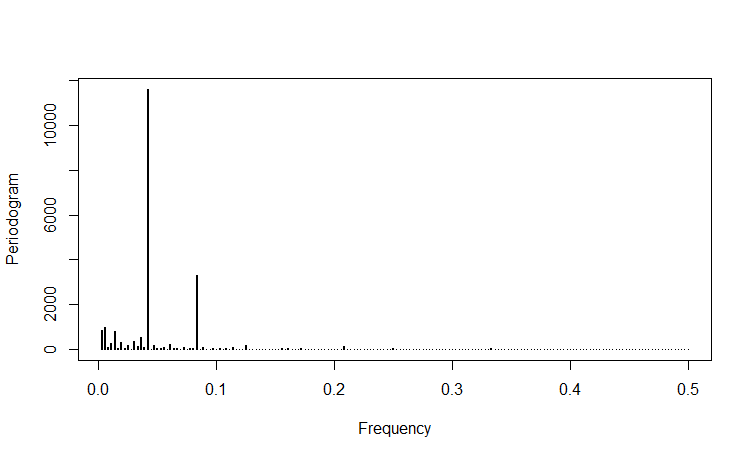
\includegraphics[width=0.8\textwidth]{figures/forecasting/periodogram_July_2014.png}
	\caption{Periodogram of hourly day ahead prices of Nord Pool Spot, Helsinki from July 7th to July 21st in 2014}
	\label{fig:periodogram_July_2014}
\end{figure}

After successfully determine meaningful seasonalities and their resulting periods from the dataset this information can be used to build forecast models that consider the respective seasonal periods in the model generation process. 



\subsection{Seasonal decomposition}

Seasonal decomposition describes the process of decomposing a given time series into its components which are trend, seasonal or cyclic and irregular components. Decomposition is done by applying the STL model to the time series and extracting the above mentioned components where STL is defined as Seasonal-Trend decomposition procedure based on Loess \cite{cleveland1990stl}. 

The decomposition of a time series can be formalized as follows \cite{cleveland1990stl}: 

	\[ Y_v = T_v + S_v + R_v \]
	
where $Y_v$ denotes the original time series, $T_v$ the trend component, $S_v$ the seasonal component and $R_v$ the remainder component. $v \in \{ 1,\ldots,N \}$ denotes an individual time stamp in the series where $N$ is the number of unit time stamps in the time series. 

A sample seasonal decomposition of hourly time series is depicted in Figure \ref{fig:stl_decomposition_July_2014}. 

\begin{figure}[htbp]
	\centering
		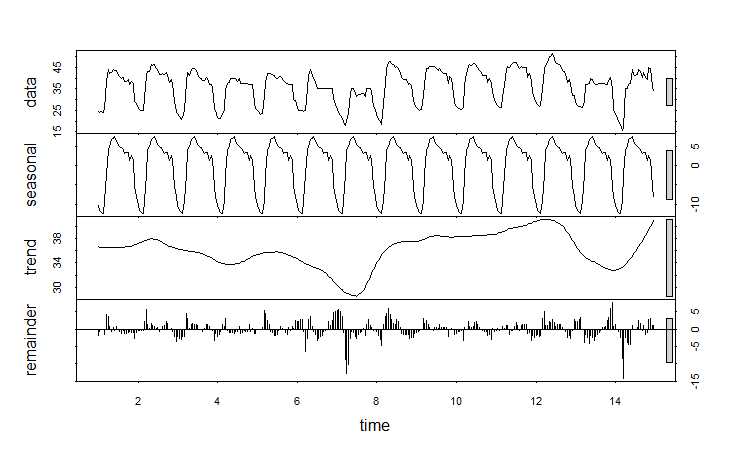
\includegraphics[width=1.00\textwidth]{figures/forecasting/stl_decomposition_July_2014.png}
	\caption{STL decomposition of hourly day ahead time series, Nord Pool Spot, Helsinki from July 7th to July 21st in 2014}	
	\label{fig:stl_decomposition_July_2014}
\end{figure}

The plot consists of four rows with each row containing a different time series component. 
The first row shows the original time series with hourly prices over a time period of two weeks. There are evident daily and weekly seasonal periods visible in the time series. Daily seasonality can be observed by the repetitive pattern of highs and lows over each day whereas weekly seasonality is evident due to the recognizable decline of prices towards the end of each week. 

The second row represents the extracted daily seasonal component which depicts the daily variation in prices. STL is only capable of extracting a single seasonality pattern. In case both daily and weekly seasonal periods should be extracted a BATS or TBATS model can be used (these models are discussed later in this section). 

In the third row the trend component is displayed. It shows a seemingly repetitive pattern over one week, which denotes the weekly seasonal period observable from the original time series. 

Finally in the last row the remaining irregular component is shown which contains all remaining variations in the time series. 

The grey bars at the right hand side of each plot aim to provide a relative comparison of scales over all plots, i.e.~the value range of the trend component is equivalent with the value range of about one third of the original time series. 




\subsection{Forecast models}

\subsubsection{BATS and TBATS}

In case of multiple seasonality periods can be done by applying a BATS or TBATS model to the time series and extracting the components \cite{de2011forecasting}. 

Both models are able to handle multiple seasonalities in the data, i.e.~considering both daily and weekly seasonal periods where TBATS models are capable of modeling non-integer periods as well (e.g.~365.25 for annual seasonality). 











\section{Model generation}





\section{Model selection algorithm}



\section{R / Java Simulation Framework}



\section{Forecast model evaluation}





%  Generated from R function getRMSEResults: Get results from forecast simulation 
% -----------------------
% Get results from forecast simulation for the given location
% over a time range of 3 years, generate models in intervals of 1 week
% with 2,3 and 4 weeks of trainings data periods
% 5 locations are available from the forecast simulation (Application server):
%  1) Hamina, locationId 1, DA
%  2) St.Ghislain, locationId 2, DA
%  3) Portland, locationId 4, RT
%  4) Richmond, locationId 6, RT
%  5) Hatfield, locationId 8, RT






%%%  General results - all numbers  %%%


Four simulations have been run for four different locations over three years of energy price data. 
For each of these locations three different training periods have been evaluated: two weeks, three weeks and four weeks. 
Each of these simulations is evaluated for five different accuracy measures: 

\begin{itemize}
	\item Mean error (ME)
	\item Mean absolute error (MAE)
	\item Root mean squared error (RMSE)
	\item Mean percentage error (MPE)
	\item Mean absolute percentage error (MAPE)
\end{itemize}

In addition, each of these error measures has been evaluated for ten different forecast horizons (in hours): 
1, 3, 6, 12, 18, 24, 36, 48, 96, 168. 

In the tables below results are shown aggregated by forecast horizon for each accuracy measure. Each table depicts a different training period for the given location. 



\subsection{Forecast evaluation results}

% latex table generated in R 3.1.1 by xtable 1.8-2 package
% Mon Mar 07 23:15:14 2016
\begin{table}[ht]
\centering
\begin{tabular}{rrrrrrr}
  \hline
 & mean & ses & holts & holtwinters & arima & tbats \\ 
  \hline
2 weeks & 14.55 & 11.60 & 62.76 & 73.65 & 10.23 & 8.19 \\ 
  3 weeks & 14.78 & 11.60 & 62.90 & 74.02 & 9.53 & 8.59 \\ 
  4 weeks & 14.99 & 11.60 & 63.23 & 85.06 & 9.26 & 8.44 \\ 
   \hline
\end{tabular}
\caption{Results of evaluation for Hamina, Nord Pool Spot (DA)} 
\end{table}


% latex table generated in R 3.1.1 by xtable 1.8-2 package
% Mon Mar 07 23:15:14 2016
\begin{table}[ht]
\centering
\begin{tabular}{rrrrrrr}
  \hline
 & mean & ses & holts & holtwinters & arima & tbats \\ 
  \hline
2 weeks & 17.07 & 15.23 & 127.13 & 186.82 & 13.49 & 1.27E+50 \\ 
  3 weeks & 17.40 & 15.27 & 128.05 & 190.21 & 12.94 & 11.60 \\ 
  4 weeks & 17.59 & 15.30 & 127.03 & 186.37 & 12.87 & 2.49E+36 \\ 
   \hline
\end{tabular}
\caption{Results of evaluation for St.Ghislain, Belpex (DA)}
\end{table}
% latex table generated in R 3.1.1 by xtable 1.8-2 package
% Mon Mar 07 23:15:14 2016
\begin{table}[ht]
\centering
\begin{tabular}{rrrrrrr}
  \hline
 & mean & ses & holts & holtwinters & arima & tbats \\ 
  \hline
2 weeks & 24.22 & 23.61 & 235.84 & 407.06 & 24.03 & 5.45E+16 \\ 
  3 weeks & 24.14 & 23.56 & 238.92 & 686.95 & 22.26 & 1.64E+18 \\ 
  4 weeks & 24.68 & 23.32 & 268.10 & 437.85 & 21.91 & 2.18E+32 \\ 
   \hline
\end{tabular}
\caption{Results of evaluation for Portland, ISO-NE (RT)}
\end{table}
% latex table generated in R 3.1.1 by xtable 1.8-2 package
% Mon Mar 07 23:15:14 2016
\begin{table}[ht]
\centering
\begin{tabular}{rrrrrrr}
  \hline
 & mean & ses & holts & holtwinters & arima & tbats \\ 
  \hline
2 weeks & 14.47 & 15.17 & 148.54 & 322.41 & 15.03 & 7.57E+13 \\ 
  3 weeks & 14.46 & 15.23 & 147.77 & 318.61 & 14.14 & 13.46 \\ 
  4 weeks & 14.42 & 15.29 & 148.67 & 357.82 & 14.11 & 5.44E+108 \\ 
   \hline
\end{tabular}
\caption{Results of evaluation for Richmond, PJM (RT)}
\end{table}



